\documentclass{article}

\usepackage{amsfonts}
\usepackage{amsmath}

\usepackage[T1]{fontenc}

\usepackage{graphicx}
\usepackage{caption}
\usepackage{array}

\usepackage{csquotes}
\usepackage[
    backend=biber,
    style=alphabetic,
    sorting=ynt
]{biblatex}
\addbibresource{reffs.bib}

\usepackage{graphicx}
\usepackage{caption}
\usepackage{array}

\usepackage{subfigure}

\usepackage[french]{babel}

\newcommand{\subf}[2]{%
    \begin{tabular}[t]{@{}c@{}}%
        #1 \\
        \footnotesize #2%
    \end{tabular}%
}

\fboxsep=0mm
\fboxrule=1pt

\usepackage{geometry}
\usepackage{pgfplots}
\pgfplotsset{width=10cm,compat=1.9}

% We will externalize the figures
\usepgfplotslibrary{external}
\tikzexternalize
\pgfplotsset{width=7cm,compat=1.18}

\title{Bruits à variation spatiale en temps réel}
\author{Arthur Chateauneuf}
\date{\today}

\begin{document}

% ---------------------------- BEGIN FIRST PAGE
\begin{titlepage}

    \newcommand{\HRule}{\rule{\linewidth}{0.5mm}}
    \center

    % ---------------------------- UNIV

    \textsc{\LARGE Université de Montpellier}\\[0.2cm]
    \textsc{\LARGE Faculté des Sciences}\\[0.2cm]
    \textsc{\Large Master 2 Informatique}\\[0.2cm]
    \textsc{\Large Parcours IMAGINE}\\[1.0cm]

    % ---------------------------- TITLE

    \HRule \\[0.5cm]
    { \LARGE \bfseries  Bruits à variation spatiale en temps réel}\\[0.5cm]
    \HRule \\[0.5cm]

    % ---------------------------- MODULE

    \textsc{\large Mémoire de stage — HAI002I}\\[1.5cm]

    % ---------------------------- NOMS

    \textsc{\large Effectué au LIRMM}\\[0.2cm]
    \textsc{\large du 27/01/2025 au 25/07/2025}\\[0.2cm]
    \textsc{\large par Arthur CHATEAUNEUF}\\[1cm]

    \textsc{\large Encadrant industriel : M. Nicolas LUTZ}\\[0.2cm]
    \textsc{\large Encadrant universitaire : M. Eric BOURREAUI}\\[1.0cm]

    % ---------------------------- LOGO

    
\includegraphics[width=.3\linewidth]{logo/UM.png}
    \hspace{0.5cm}
    
\includegraphics[width=.25\linewidth]{logo/LIRMM.png}
\end{titlepage}

\clearpage

\tableofcontents

\clearpage

\section{Introduction}

\subsection{Contexte du stage}

Dans le cadre de mon Master Informatique, j'ai effectué un stage industriel
encadré par Nicolas Lutz au Laboratoire d'Informatique, de Robotique et de
Microélectronique de Montpellier (LIRMM). J'ai travaillé au sein du département
informatique dans l'équipe ICAR sur le sujet des bruits à variation spatiale en
temps réel.

\subsection{Contexte technique et méthode de travail}

Lors de ce stage, j'ai travaillé sur ma propre base de code en utilisant
Vulpine, mon propre moteur de jeu et d'applications interactives que j'ai eu
l'occasion de développer dans le cadre de mon parcours académique. Je possédais
ainsi une forte base technique et une connaissance approfondie de mes outils
dès le début de mon travail de recherche. J'ai travaillé en collaboration
étroite avec mon maitre de stage Nicolas Lutz, qui m'a initié au monde de la
recherche et au sujet de mon stage. Nous faisions le point plusieurs fois par
mois pour que je lui présente mes avancées et qu'il me propose des pistes
d'améliorations.

Durant l'ensemble de mon stage, j'ai eu l'occasion de rencontré de nombreux
chercheurs, doctorants et stagiaires. J'ai participé régulièrement à des
réunions d'équipes où j'ai eu l'occasion d'assister à la présentation de leur
travail. J'ai également présenté mon sujet de stage devant ces mêmes équipes.

\subsection{Problématique}

En informatique graphique, un bruit est un processus stochastique (ou fonction
aléatoire) permettant de créer des variations de motifs infinis, le plus
souvent en deux ou trois dimensions, utilisé pour la création d'effets visuels
complexes comme la simulation de flammes ou d'océans. Cependant, la majorité
des bruits utilisés sont dits stationnaires, cela signifie que leurs attributs
statistiques (variance, moyenne, histogramme...) n'évoluent pas en fonction de
l'espace ou des réalisations.

Il existe des solutions non stationnaires, dont un exemple est visible dans la
figure \ref{comparaison_stationnarité}, qui ne sont cependant pas utilisables
dans un contexte temps-réel. De telles méthodes nécessitent des pré-calculs
lourds et la sauvegarde de résultats à l'intérieur d'une texture matricielle.
L'un des travaux les plus notables et récents dans cette optique est One Noise
to Rule Them All \cite{One_Noise}, publié en 2024, qui présente une solution de
création de bruit à variation spatiale généré par un réseau de neurone.

Si une méthode permettant d'obtenir des résultats similaires en temps réels
était trouvée, cela ouvrirait les portes à l'utilisation de bruits à variation
spatiales dans des contextes procéduraux, non bornés, animés ou même
interactifs. Une telle avancée améliorerait la qualité et la modularité des
outils utilisés dans de nombreux domaines comme le jeu vidéo ou la modélisation
3D.

Une fois familiarisé avec les concepts de technique et de recherche
nécessaires, ma mission lors de ce stage a été d'explorer des solutions
permettant de combiner des bruits stationnaires afin d'obtenir une sortie non
stationnaire. Premièrement en utilisant le pavage et mélange\cite{HPnoise} et
ensuite en utilisant l'opérateur de mélange Mix-Max\cite{mixmax}.

\begin{figure}
    \centering
    \begin{tabular}{cc}
        \subf{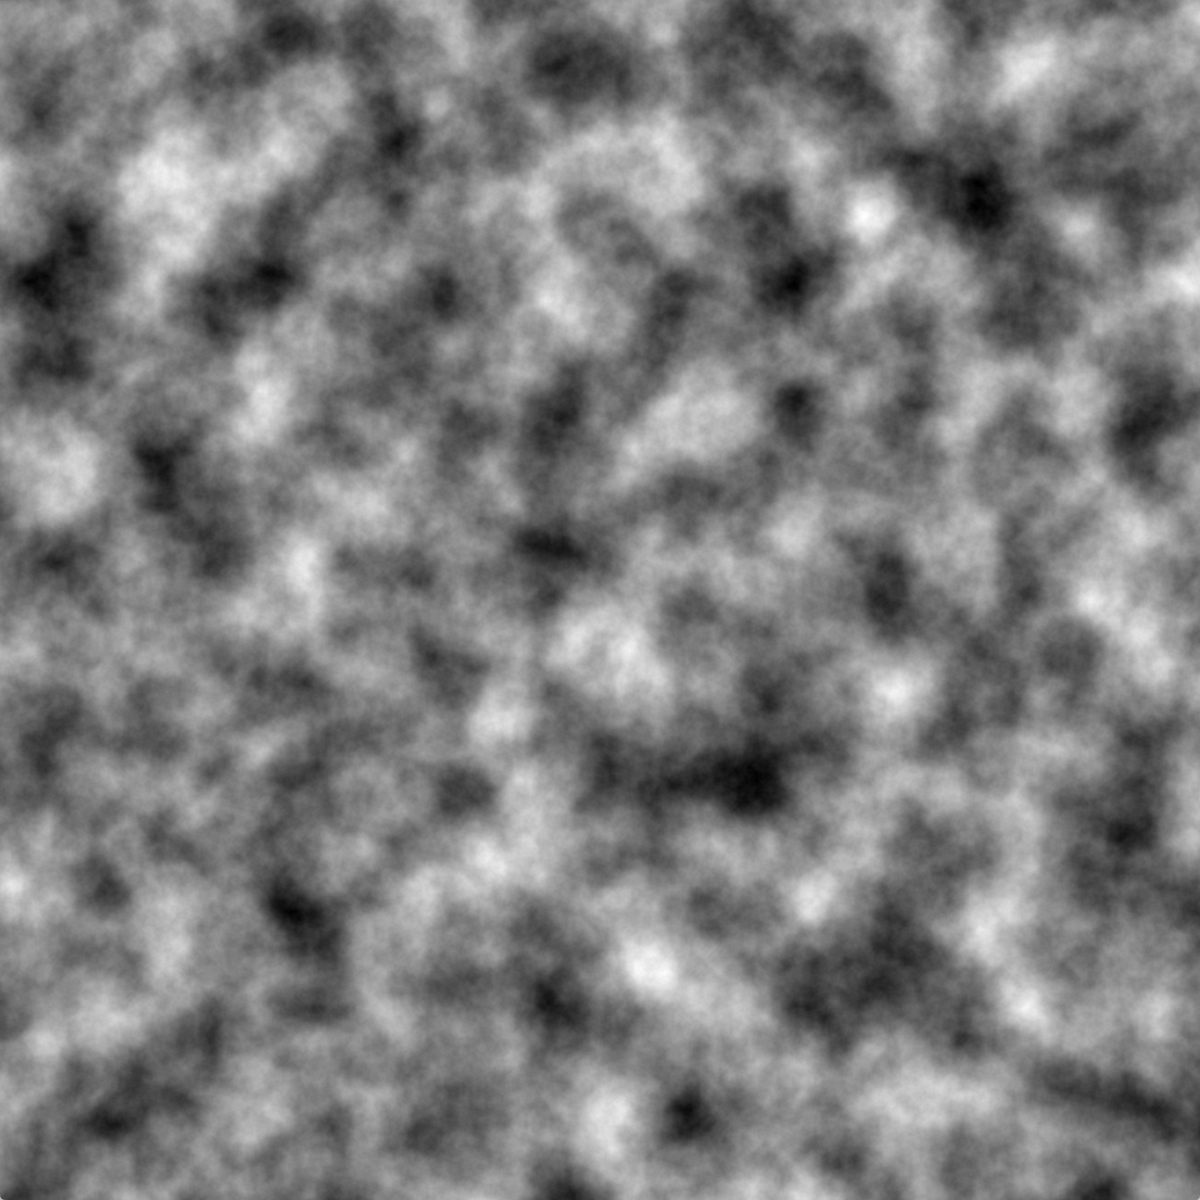
\includegraphics[width=0.5\textwidth]{fig/Perlin.png}}
        {Bruit de Perlin                   \\ Stationnaire}

        \subf{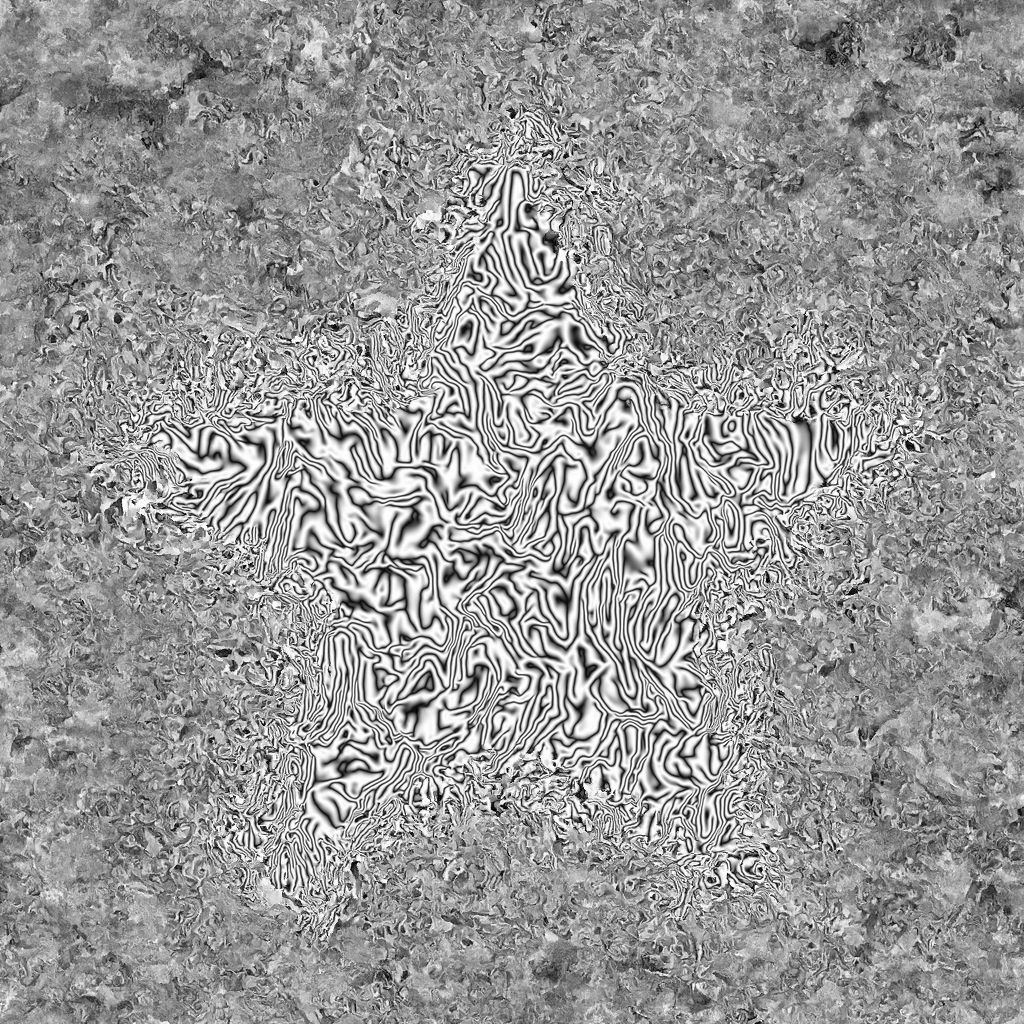
\includegraphics[width=0.5\textwidth]{fig/OneNoise.png}}
        {Mélange de Bruit \cite{One_Noise} \\ Non stationnaire}

    \end{tabular}
    \caption{Comparaison visuelle entre un bruit stationnaire et non stationnaire. De claires variations statistiques sont visibles dans les motifs produit par la méthode non stationnaire.}
    \label{comparaison_stationnarité}
\end{figure}

\newpage

\section{État de l'art}

\subsection{State of the Art in Procedural Noise Functions}

Mon travail a commencé avec la lecture de State of the Art in Procedural Noise
Functions \cite{SOA_Noise}, un état de l'art avancé sur la conception de bruits
procéduraux temps réel. Ce papier fait d'abord état d'un fait dans l'évolution
des capacités des processeurs graphique : l'efficacité des calculs évolue à un
rythme plus grand que celle de la mémoire. Cela signifie que l'empreinte
mémoire des algorithmes est de plus en plus déterminante dans leur rapidité.
Cela permet à des méthodes auparavant trop couteuses en calculs de devenir de
bonnes alternatives, parfois même préférables.

L'utilisation de bruits procéduraux fait partie intégrante de ces évolutions
dans l'informatique graphique. Les bruits sont définis plus formellement comme
des processus combinant plusieurs signaux de façon pseudo-aléatoire
\cite{SOA_Noise}. Le terme de "bruit" venant, quant à lui, de l'utilisation
originelle de ces techniques dans le cinéma et les images de synthèse, qui
servaient à recréer de façon rapide des irrégularités dans des signaux visuels
tels que des textures.

Ces techniques sont le plus souvent utilisées en pré-calculs. Leurs résultats
sont ainsi stockés dans la mémoire sous forme de textures matricielles en deux
ou trois dimensions. Cependant, cette méthode garde les limitations techniques
de l'utilisation de données pré-calculés. Les textures sont ainsi bornées,
possèdent une résolution limitée et augmentent l'empreinte mémoire à chaque
échantillonnage. L'alternative est de calculer ces processus pendant leur
rendu, pour chaque fragment de chaque image devant être calculé. Ces méthodes
sont qualifiées de procédurales, car elles produisent des infinités de motifs
non périodiques, pseudo-aléatoires et continus.

L'absence de dépendance sur des données discrétisées diminue grandement
l'empreinte mémoire tout en offrant la possibilité de calculer en temps réel
des itérations différentes de chaque bruit. Le rendu résultant peut ainsi
réagir à n'importe quelle influence extérieure, le rendant animable ou
interactif. Les plus grands avantages des processus procéduraux sont leur
résolution et leur taille infinies, s'adaptant en temps réel aux besoins du
rendu.

Les difficultés du calcul en temps réel sont également abordées. Tous les
éléments procéduraux doivent être filtrés analytiquement lors du rendu d'une
texture sur une surface. Cela signifie que la moyenne de leur intensité/couleur
doit être calculé sur la zone entière que couvre chaque fragment que l'on
souhaite rendre. L'un des plus grands défis de la création de bruits
procéduraux est de trouver des méthodes permettant de calculer ou d'approximer
de façon suffisamment précise ces moyennes. Sur des textures matricielles
(composés de pixels stockés en mémoire), cela se fait par l'utilisation de
mip-maps, qui sont des versions sous-échantillonnés de la texture originale.
Une telle méthode est cependant impossible avec des textures procédurales, car
aucune valeur n'est pré-calculée.

Ce papier m'a permis d'obtenir des enseignements importants pour la
compréhension de la nature des bruits procéduraux ainsi que de leur pertinence.
Il démontre également la complexité des problèmes à résoudre afin de
correctement afficher une texture matricielle sur une surface.

\subsection{One Noise to Rule Them All: Learning a Unified
    Model of Spatially-Varying Noise Pattern}

Par la suite, je me suis intéressé aux avancées en création de processus non
stationnaires. La publication la plus pertinente sur cette piste est One Noise
to Rule Them All \cite{One_Noise}, un modèle de génération de bruits
procéduraux non stationnaires.

La méthode proposée dans ce papier utilise un réseau de neurones entrainé sur
une série d'échantillons de bruits procéduraux stationnaires. Ce dernier est
capable de générer des bruits non stationnaires en mélangeant des patternes de
plusieurs bruits. Cette méthode permet ainsi de combiner n'importe quel bruit
pré-existant en une infinité de sorties non stationnaires. Les variations
spatiales sont apportées grâce à une carte de mélange donnée par l'utilisateur.
L'objectif est alors de transformer une entrée non stationnaire simple en une
infinité de sorties complexes. Cela permet la création de patternes possédant
des attributs uniques variant spatiallement de façon logique et équilibré.

Cet algorithme ne permet cependant pas de générer des entrées en temps réel,
car il nécéssite l'utilisation d'un réseaux de neuronne qui stocke des
résultats discrétisés. Le bruit généré est ainsi borné, non continue et ne peut
pas réagir aux influences extérieures.

Ce papier montre que le mélange de plusieurs bruits stationnaires est un moyen
efficace d'obtenir les résultats que je recherche. J'ai ainsi décider de
m'inspirer de leur approche en explorant les méthodes de mélange de processus
procéduraux pouvant être appliqué en temps réels. Cela nécéssite une méthode
rapide, parraléllisable, peut couteuse en mémoire et analytiquement filtrable.

\subsection{High-Performance By-Example Noise
    using a Histogram-Preserving Blending Operator}

La première piste d'algorithme de mélange que j'ai étudié était le pavage et
mélange, présenté dans le papier High-Performance By-Example Noise using a
Histogram-Preserving Blending Operator \cite{HPnoise} publié en 2018. Il y est
décrit un système de pavage, pouvant être rectangulaire ou hexagonale,
permettant de représenter de façon infinie et non répétitif une texture
discrétisée sur une surface 3D.

Chaque fragment que l'on shouaite calculé est interpolé entre trois instances
de la texture originelle, chacune ayant une rotation et une translation
différente. La sortie obtenue est ainsi majoritairement composé de couleurs
interpollés. Afin de réduire le flou et l'introduction de teintes non présentes
dans la texture originale, deux équations de mélange sont proposés. La
première, applicable en temps réel, préserve la moyenne ainsi que la variance
de l'entrée. La seconde, quant à elle, nécéssite une grande quantité de
pré-calculs et une multitude de défis techniques mais permet de préserver
l'histogramme en plus de la variance.

Cette méthode pourrait servir à mélanger des bruits procéduraux et à créer des
transitions respectant certaines propriétés statistiques, améliorant la qualité
visuelle de mélanges entre deux bruits. La première équation de préservation de
la variance permettrait d'appliquer cette amélioration en temps réel.

\subsection{Mix-Max: A Content-Aware Operator for Real-Time Texture Transitions}

L'opératuer Mix-Max \cite{mixmax} offre également une piste très prométeuse
pour le mélange de bruits. Proposée en 2024, cette méthode a été conçus pour
mélanger des textures matricielles représentant des matériaux opaques. Cette
méthode permet d'obtenir des transitions nettes et naturelles entre une
infinité de textures, tout en étant filtrable analytiquement et utilisable en
temps réel. Cependant, cette méthode entraine l'échantillonage de plusieurs
textures pour chaque entrée, augmentant l'empreinte mémoire par rapport à un
mélange linéaire simple.

Ces résultats sont obtenus grâce à l'utilisation d'une carte de priorité, crée
par l'utilisateur selon ses besoins, qui biaise le mélange en faveur ou contre
sa texture attribué. Si la texture de prioritée est obtenue à partir du contenu
de la texture de couleur, on obtient alors un opérateur de mélange sensible au
contenu. Les résultats de cette méthode sont inédits. Si l'on shouaite
mélanger, par exemple, une texture de brique et de mousse, il est possible de
faire se répandre la mousse en priorité entre les creux des briques. Cet
opérateur offre des paramétres tels que le choix des textures d'entrées, de
leur priorité, de leur poids de mélange ainsi que la netteté de la transition,
le tout en étant analytiquement filtrable. Cependant, il n'est utilisable
qu'avec des textures matricielles et nécéssite l'utilisation d'au moins deux
autres textures de support pour chaque entrée que l'on shouaite mélanger.

L'opérateur Mix-Max, s'il est étendue aux bruits procéduraux, permettrait
d'obtenir un mélange de patternes respectant leur contenus et possédaznt toutes
les propriétés nécéssaires à l'utilisation en temps réel. Cela permettrait de
simuler des résulats théoriquement proches de One Noise to Rule Them All.

\newpage

\section{Mélange de processus stationnaires}

\subsection{Texture, Bruit et empreinte}

Afin de mettre en place des techniques de mélanges de bruits procéduraux, il
est nécéssaire de définir les aspects théoriques concernés. Premièrement, un
processus $\mathcal{P}$ est une fonction associant un interval de valeurs $V$
de dimension $n$ à un espace d'échantillonage $\mathbf{u}$ de dimension $m$ :

\begin{equation}\centering\label{Def processus}
    \mathcal{P} : \mathbf{u} \rightarrow V \mid \mathbf{u} \subset \mathbb{R}^m \land V \subset \mathbb{R}^n
\end{equation}

Une texture $\mathcal{T}$ est un processus dont l'interval de valeur est
compris entre 0 et 1 pour chaque dimensions, et dont l'espace d'échantillonage
est deux-dimensionnel :

\begin{equation}\centering\label{Def Texture}
    \mathcal{T} : \mathbf{u} \rightarrow [0, 1]^n \mid \mathbf{u} \subset \mathbb{R}^2
\end{equation}

Une texture matricielle $\mathcal{T}_m$ est une texture possèdant des valeurs
composés par l'interpolation d'un interval discret $\mathbb{D}$, représentant
l'ensemble des combinaisons de pixels stockés dans la texture. Un tel processus
possède un espace d'échantillonage borné dans l'interval $[0, 1]$ :

\begin{equation}\centering\label{Def Texture Matricielle}
    \mathcal{T}_m : [0, 1]^2 \rightarrow Interp (\mathbb{D}) \mid \mathbb{D} \subset [0, 1]^n
\end{equation}

Une texture procédurale $\mathcal{T}_p$ est une texture possèdant des valeurs
continues et pouvant être échantillonée sur $\mathbb{R}^2$ :

\begin{equation}\centering\label{Def Texture Procédurale}
    \mathcal{T}_p : \mathbb{R}^2 \rightarrow [0, 1]^n
\end{equation}

Un bruit $\mathcal{B}$ est une texture aléatoire associant des intensités
scalaires non périodiques \cite{SOA_Noise} à son espace d'échantillonage. Un
bruit peut ainsi également être matriciel ou procédural. De plus, il possède un
espace de réalisation. Une réalisation $\omega$ est un tirage du bruit
aléatoire.

\begin{equation}\centering\label{Def Bruit}
    \mathcal{B} : \mathbf{u}, \omega \rightarrow [0, 1]
\end{equation}

\begin{equation}\centering\label{Def Bruit Non périodique}
    \forall t, \; \exists x \in \mathbf{u} \mid t+x \in \mathbf{u} , \; \mathcal{B}(x) \neq \mathcal{B}(x + t) \sim \textit{non périodicité}
\end{equation}

L'empreinte moyenne $\mathcal{T}(\mathbb{P})$ d'un processus $\mathcal{P}$ sur
une zone $\mathbb{P}$ permet de connaitre la moyenne de toutes les valeurs que
le processus prend sur cette zone :

\begin{equation}\centering\label{Def Empreinte}
    \mathcal{P}(\mathbb{P}) = \frac{1}{area(\mathbb{P})} \int_{\mathbb{P}} \mathcal{T}(\mathbf{u}) d \mathbf{u}
\end{equation}

Toute méthode de filtrage analytique d'une texture doit approximer l'empreinte
moyenne pour obtenir un rendu satisfaisant \cite{SOA_Noise}.

\subsection{Opérateur de mélange}

Un opérateur de mélange $\mathcal{M}$ est un processus représentant le mélange
entre deux textures $\mathcal{T}_1, \mathcal{T}_2$ pondéré par les poids de
mélange $v_1, v_2$. Le mélange entre deux texture doit tendre vers les valeurs
de chaque entrées lorsque son poids devient maximal. Un tel system obéit aux
équations \ref{Propriété Alpha} et \ref{Propriété Mélange} :

\begin{equation}\centering\label{Propriété Alpha}
    v_i \in [0, 1] ,\, v_1 + v_2 = 1
\end{equation}

\begin{equation}\centering\label{Propriété Mélange}
    \lim_{v_i \rightarrow 1} \mathcal{M}(\mathbf{u}) = \mathcal{T}_i(\mathbf{u})
\end{equation}

L'opacité $w_i$ d'une texture $\mathcal{T}_i$ correspond à son importance
finale dans le mélange, elle répond à l'équation \ref{Propriété Opacité} :

\begin{equation}\centering\label{Propriété Opacité}
    \mathcal{M}(\mathbf{u}) = w_1 \mathcal{T}_1(\mathbf{u}) + w_2 \mathcal{T}_2(\mathbf{u})
\end{equation}

Un mélange est dit équilibré si l'espérance de l'opacité de chaque texture est
égal à son poids initial, respectant la propriété de l'équation \ref{Def
    Mélange Equilibré} :

\begin{equation}\centering\label{Def Mélange Equilibré}
    \mathbb{E}[w_i] = v_i
\end{equation}

Le mélange linéaire $\mathcal{M}^{lin}$ est la méthode la plus simple et
répandue de mélanger deux texture. L'opacité est directement égale au poids de
mélange initaux :

\begin{equation}\centering\label{Mélange Linéaire}
    \mathcal{M}^{lin} = v_i \mathcal{T}_1(\mathbf{u}) + v_2 \mathcal{T}_2(\mathbf{u})
\end{equation}

\subsection{Stationnarité}

Un bruit, qui est assimilable à une variable aléatoire $X$, est dit
stationnaire à l'ordre $n$ lorsque son moment d'ordre $n$ est constant sur
chaque réalisation à n'importe quelle coordonée $\mathbf{u}$. En pratique, les
ordres de moment 1 et 2, respectivement la moyenne $\mathbb{E}$ et la variance
$Var(X)$, sont suffisantes à prouvés \cite{SOA_Noise}. Un bruit stationnaire
respecte aisni l'équation \ref{Def Stationnaire} :

\begin{equation}\centering\label{Def Stationnaire}
    \begin{split}
        \mathbb{E}[X(\mathbf{u})] &= constante
        \\
        Var[X(\mathbf{u})] &= constante
    \end{split}
\end{equation}

Inversement, un bruit n'est pas stationnaire si sa moyenne et sa variance sur
l'ensemble des réalisations dépend de la coordonée $\mathbf{u}$. Il est ainsi
possible de parler de variation spatiale \cite{One_Noise} dans les motifs de la
texture. Dans le cas d'un mélange de textures, même si ces dernières sont
stationnaires, si les poids $w_1, w_2$ sont non stationnaires, alors le mélange
$\mathcal{M}$ le sera également.

\newpage

\section{Création de variation spatiale par Pavage et Mélange}

\begin{figure}
    \centering
    \begin{tabular}{ccc}
        \subf{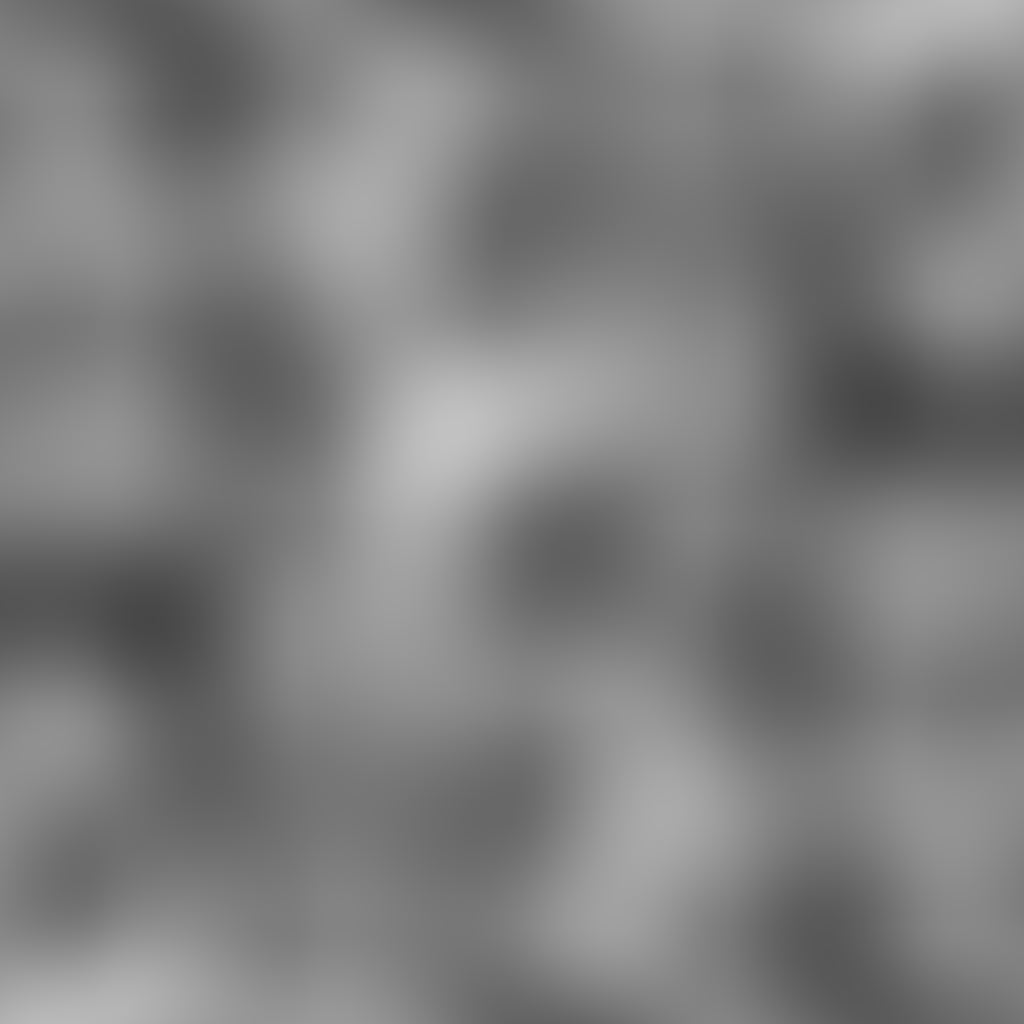
\includegraphics[width=0.29\textwidth]{fig/hpn/Gradient.png}}
        {$\mathcal{T}_1$                      \\\footnotesize (Stationnaire)}

        \subf{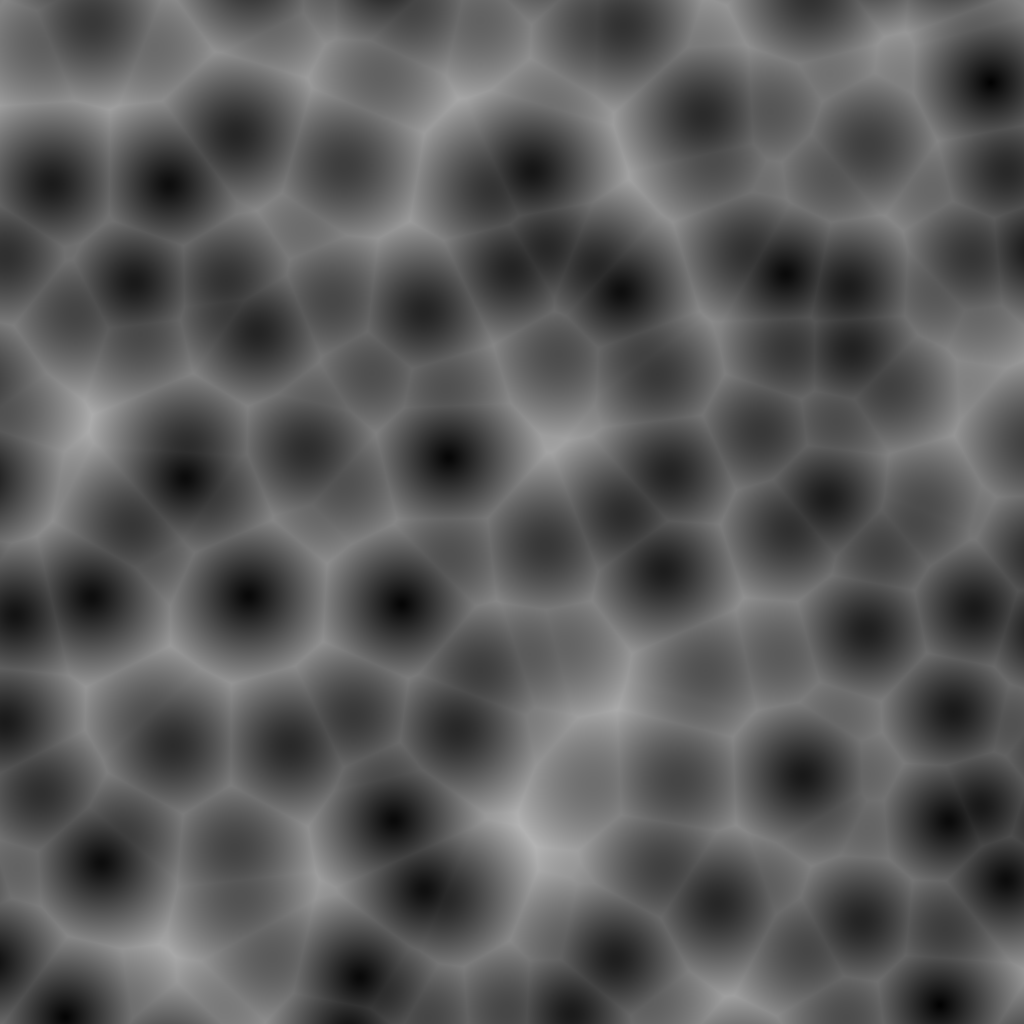
\includegraphics[width=0.29\textwidth]{fig/hpn/Voronoi.png}}
        {$\mathcal{T}_2$                      \\\footnotesize (Stationnaire)}

        \subf{
\includegraphics[width=0.29\textwidth]{fig/hpn/v.png}}
        {$v_1$ créer par pavage               \\\footnotesize (Non stationnaire)}

        \\

        \subf{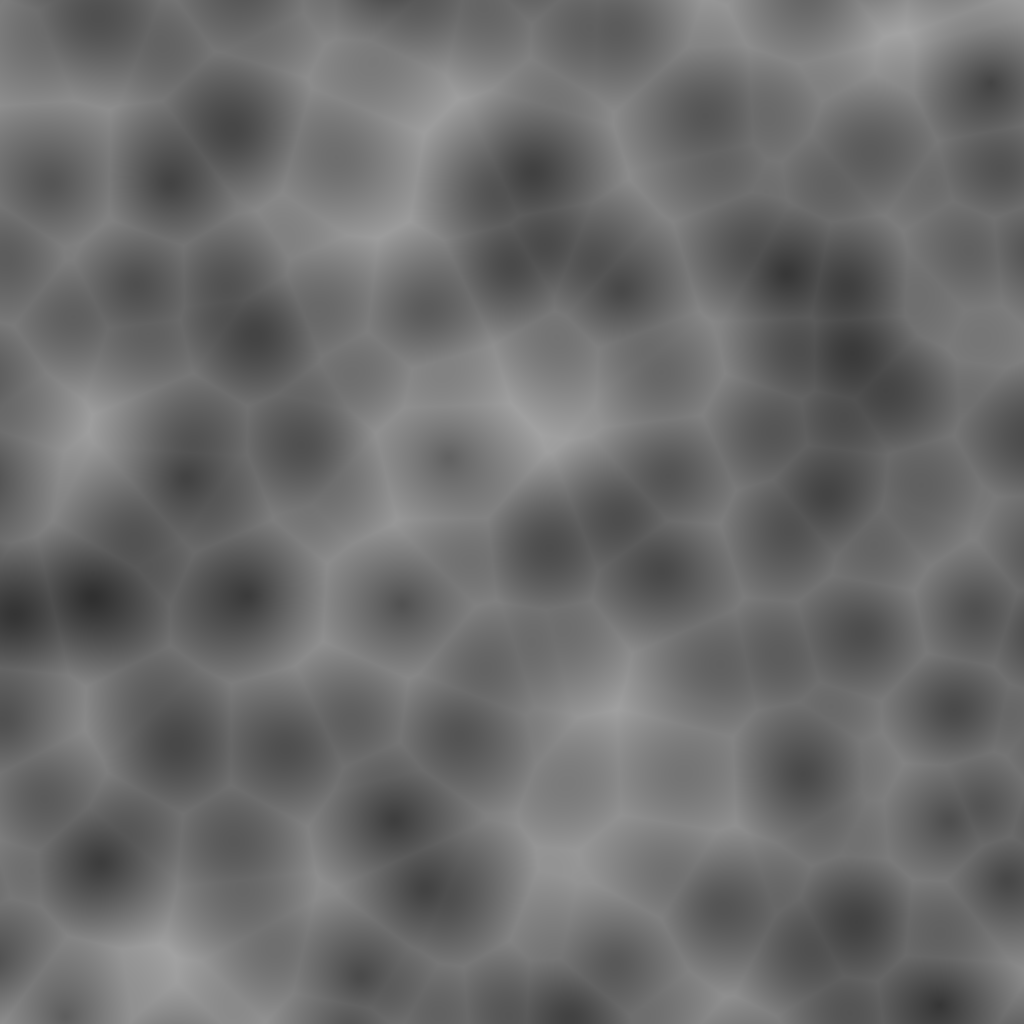
\includegraphics[width=0.29\textwidth]{fig/hpn/Linear.png}}
        {$\mathcal{M}^{lin}$ avec $v_1 = 0.5$ \\\footnotesize (Stationnaire)}

        \subf{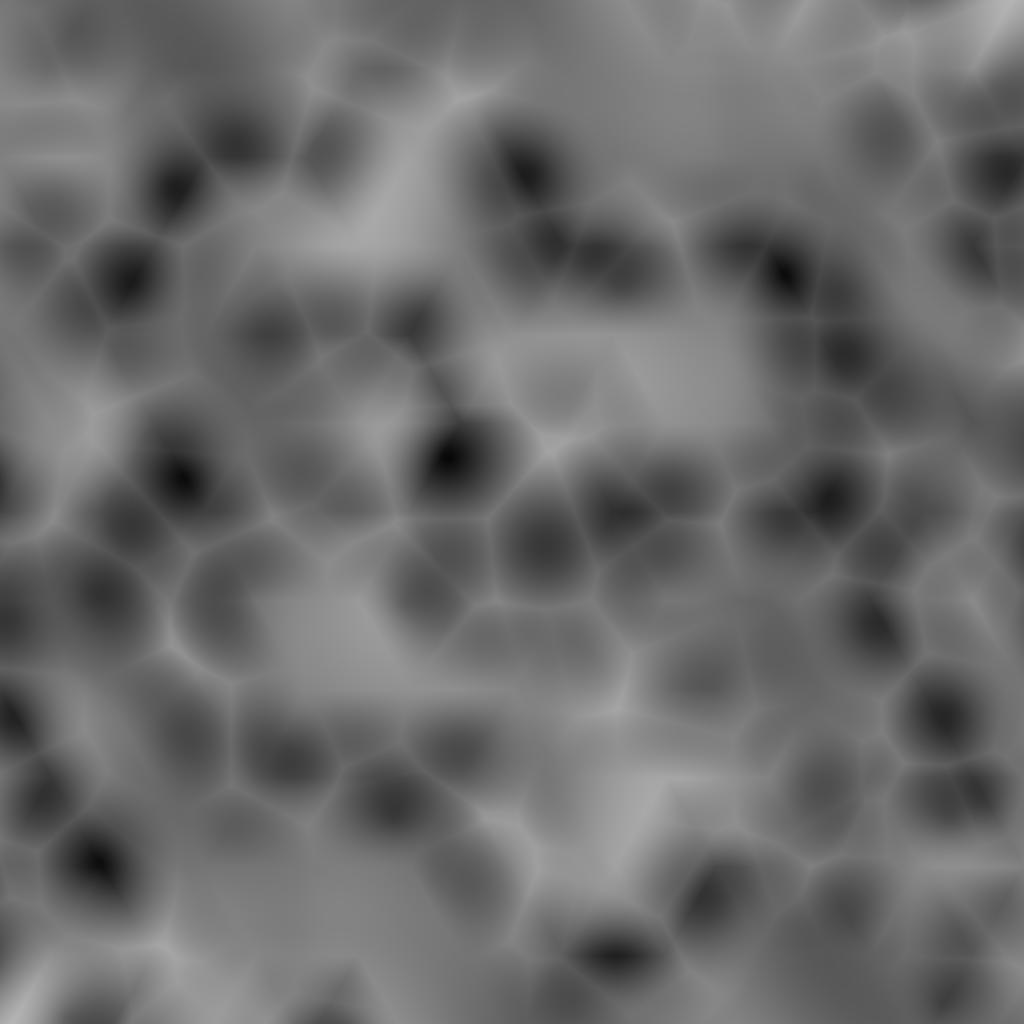
\includegraphics[width=0.29\textwidth]{fig/hpn/HPN Linear.png}}
        {$\mathcal{M}^{lin}$ avec pavage      \\\footnotesize (Non stationnaire)}

        \subf{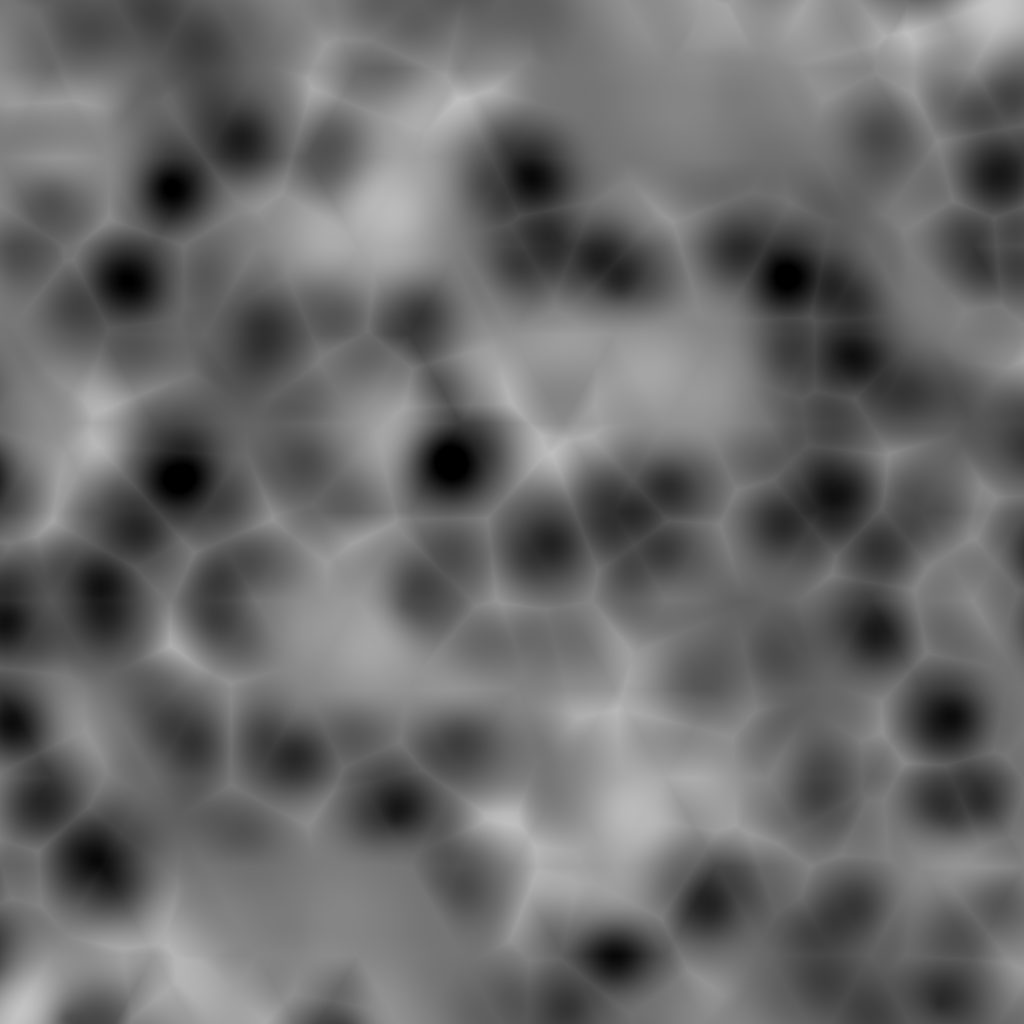
\includegraphics[width=0.29\textwidth]{fig/hpn/HPN.png}}
        {$\mathcal{M}^{cov}$ avec pavage      \\\footnotesize (Non stationnaire)}

    \end{tabular}
    \caption{Comparaison entre différentes méthodes de mélanges entre les textures $\mathcal{T}_1$ et $\mathcal{T}_2$. Le pavage apporte des variation spatiale, même avec des entrées stationnaires. Le mélange préservant la variance $\mathcal{M}^{cov}$ évite que le résultat ne tende vers une gaussienne, rendant le contraste (ou la variance) du résultat similaire à celui des entrées.
    }
    \label{Resultats_Pavage_et_Melange}
\end{figure}

\subsection{Méthode}

L'algorithme de pavage et mélange \cite{HPnoise} introduit une grille
hexagonale de pavage, ainsi qu'un opérateur de mélange permettant de préserver
la variance des entrées. Cependant ce système est utilisé sur une seule et même
texture matricielle, afin d'en faire une texture procédurale. Mon objectif est
de l'appliquer à deux bruits procéduraux différents afin d'obtenir des
patternes à variation spatiale.

Pour cela, il est nécéssaire d'attribuer à chaque céllule de la grille une
texture. L'algorithme original applique une translation et une rotation
aléatoire pour chaque céllule. Cette opération n'est pas nécéssaire car toutes
les textures utilisés sont procédurales. La variation spatiale est ainsi
apporté par le choix d'attribution des céllules. Un exemple de notre
implémentation est présenté dans la figure \ref{Resultats_Pavage_et_Melange}.

L'opérateur de mélange préservant la variance, montré dans l'équation
\ref{Mélange préservant variance}, doit également être adapté, car il utilise
l'espérance du mélange final, qui est conu dans le cas où chaque entrée
provient de la même texture, mais qui est inconnu dans mon cas d'utilisation..

\begin{equation}\centering\label{Mélange préservant variance}
    \mathcal{M}^{cov} =
    \frac{v_1\mathcal{T}_1 + v_2\mathcal{T}_2 - \mathbb{E}[\mathcal{M}^{cov}]}{\sqrt{v_1^2 v_2^2}}
    +\mathbb{E}[\mathcal{M}^{cov}]
\end{equation}

Mon apport sur cette méthode a été de trouver la valeur de l'espérence du
mélange qui satisfaisait l'équation \ref{Mélange préservant variance}. Elle est
égale à la moyenne pondérée des espérances de chaque entrée :

\begin{equation}\centering\label{Espérance mélange préservant la varance}
    \mathbb{E}[\mathcal{M}^{cov}] = v_1\mathbb{E}[\mathcal{T}_1] + v_2\mathbb{E}[\mathcal{T}_2]
\end{equation}

L'impacte de cette formule est visible sur la figure \ref{Résultats Pavage et
    Mélange}.

\subsection{Limitations}

Bien que le pavage et mélange permette d'obtenir des bruits à variation
spatiale en temps réel, la qualité des résultat varie grandement en fonction
des entrées, comme le démontre la figure \ref{Gradient Pavage et Mélange}. Des
textures nettes, par exemple, entraineront une grande perte de cohésion des
patterns. Malgré l'apport de préservation du contraste (ou de la variance) la
qualité des transition reste très proche de la méthode linéaire.

Obtenir de meilleur résultats nécéssiterait une méthode sensible aux patternes
et à l'histogramme des textures que l'on shouaite mélanger. Cela permettrait
une bonne adaptabilité à tout les types de bruits.

\begin{figure}
    \centering
    \begin{tabular}{cc}
        \subf{\fbox{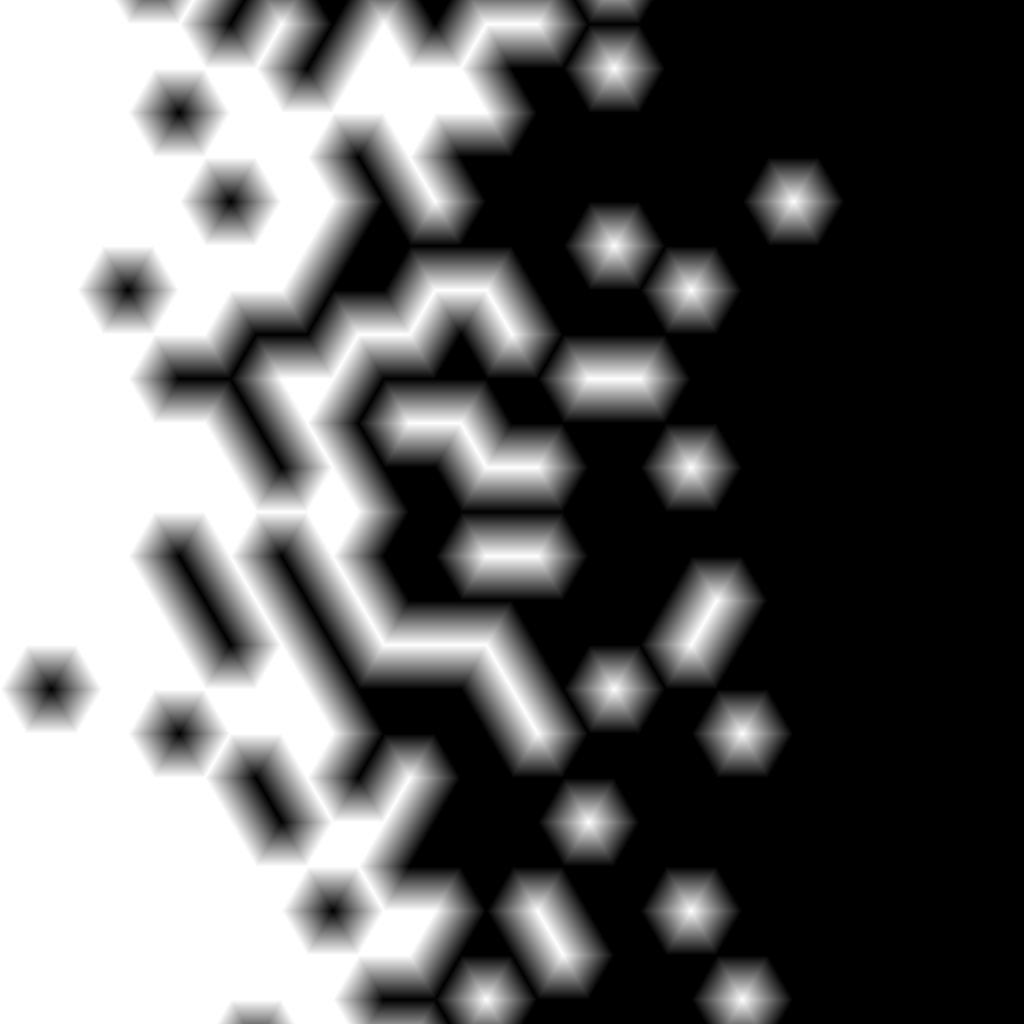
\includegraphics[width=0.4\textwidth]{fig/hpn/Gradient v1.png}}}
        {$v_1$ créer par pavage}

        \subf{\fbox{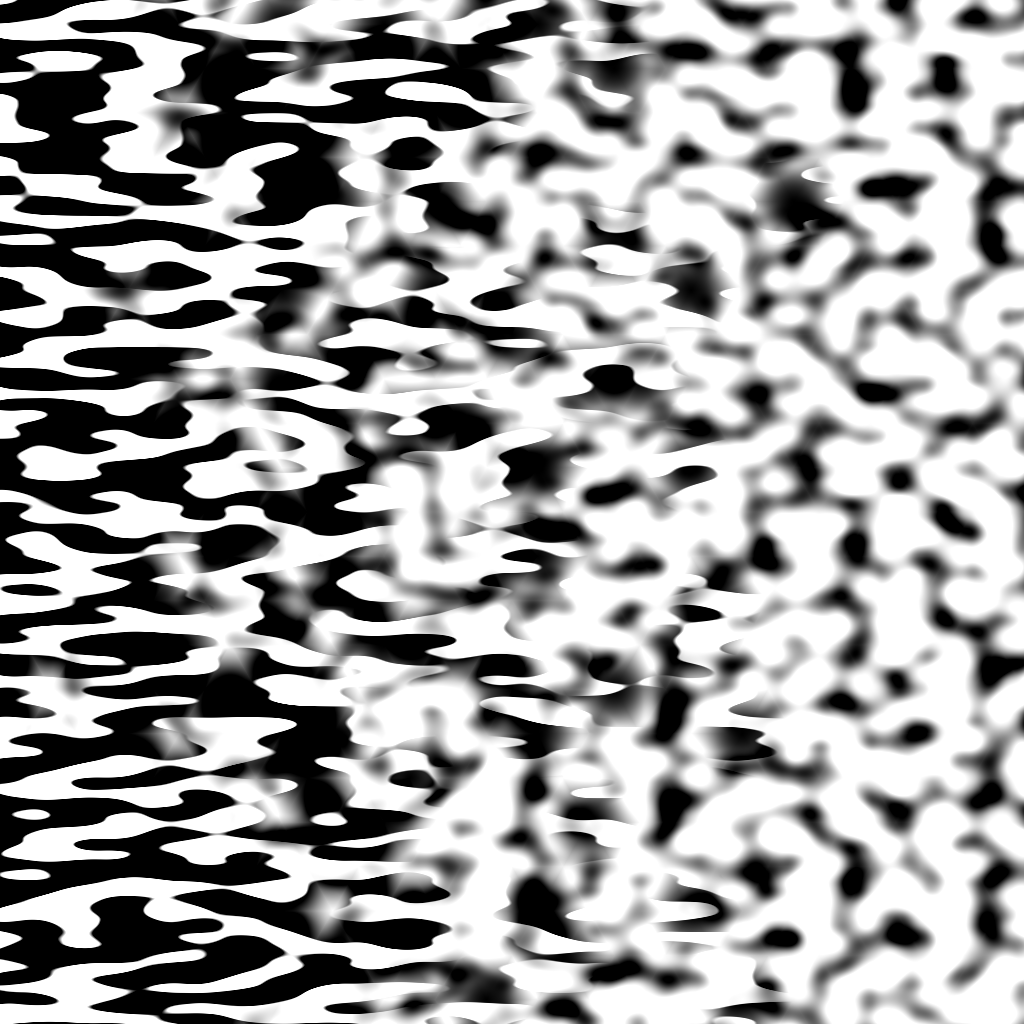
\includegraphics[width=0.4\textwidth]{fig/hpn/Gradient cov.png}}}
        {$\mathcal{M}^{cov}$}
    \end{tabular}
    \caption{Transition horizontale entre deux textures nettes en utilisant le pavage et mélange préservant la variance présenté dans l'équation \ref{Mélange préservant variance}. La pauvre qualité visuelle du résultat montre la limite de cette méthode qui ne s'adapte pas aux motifs ou à la netteté des entrées.
    }
    \label{Gradient Pavage et Mélange}
\end{figure}

\newpage

\section{Création de variation spatiale par Mix-Max}

\subsection{Motivations}

L'opérateur de mélange Mix-Max permet de créer des transitions (de textures
matircielles) paramétrables et s'adaptant au contenu de toutes les entrées
\cite{mixmax}. Son principe est de représenter les textures comme des éléments
pouvant etre soit totalement opaques, soit totalement écrasés lors du mélange.
Cette méthode est qualifiée de mélange binaire. Pour savoir quelle texture doit
être choisis à chaque endroit, des cartes de priorités $\mathcal{S}_i$ sont
attribués à chaques entrées. Pour finir, les priorités sont décalés par les
poids de mélange, rendant, par exemple, la texture $\mathcal{T}_i$ très
présente dans le mélange lorsque $v_i$ est grand. Les opacités $w_1$ et $w_2$
ainsi crées par le Mix-Max respectent l'équation \ref{Bases Mix Max}
\cite{mixmax} :

\begin{equation}\centering\label{Bases Mix Max}
    \begin{split}
        w_1(\mathbf{u}) &= \begin{cases}
            1, & \text{Si } \mathcal{S}_1(\mathbf{u})  + v_1(\mathbf{u})  > \mathcal{S}_2(\mathbf{u})  + v_2(\mathbf{u}) \\
            0, & \text{Sinon}
        \end{cases} \\
        w_2 &= 1-w_1
    \end{split}
\end{equation}

Dans son état actuel, le Mix-Max possède plusieurs limitation pour mon cas
d'utilisation. Premièrement, ce mélange n'est pas équilibré, rendant impossible
un contrôle précis de la transition. Deuxièmmement, les méthodes de filtrage
proposés ne sont compatibles qu'avec des textures matricielles.

\subsection{Priorité équilibré}

Equilibrer le Mix-Max permettrait d'obtenir une probabilité de présence de
chaque texture équivalente à son poids initial :
\begin{equation}\centering\label{Bases Mix Max équilibré}
    \begin{split}
        P(w_1 = 1) &= v_1 \\
        P(w_2 = 1) &= v_2
    \end{split}
\end{equation}
Cette propriété permettrait à n'importe quel utilisateur de contrôler précisément le niveau de présence de chaque texture.

Pour cela, il faut d'abord un socle commun entre toutes les textures de
priorités, car ces dernières peuvent posséder n'importe quel histograme ou
contenu, tant que leur moyenne est proche de $0.5$ \cite{mixmax}. Si chaque
texture de priorité subissait un applitissement d'histogramme, elles
respecteraient alors l'équation \ref{Propriété Priorité Applatie}, rendant
facilement prédictible la probaiblité de chaque résultat :
\begin{equation}\centering\label{Propriété Priorité Applatie}
    P(\mathcal{S}_i > x) = x
\end{equation}
Avec des priorités à l'histogramme plat, il est possible de trouver un décallage parfait $\Delta_i$ pour chaque priorité $\mathcal{S}_i$ qui équilibre le mélange :
\begin{equation}\centering\label{Formule Delta Mix Max Equilibré}
    \Delta_i = \frac{1}{2} sgn \left( v_i-\frac{1}{2} \right)
    \left( 1 - \sqrt{1 - 2 \left| v_i-\frac{1}{2} \right|} \right)
\end{equation}
Le résultat de l'application de cette formule est visible sur la figure \ref{Résultats Priorités}.

\clearpage

\begin{figure}
    \centering
    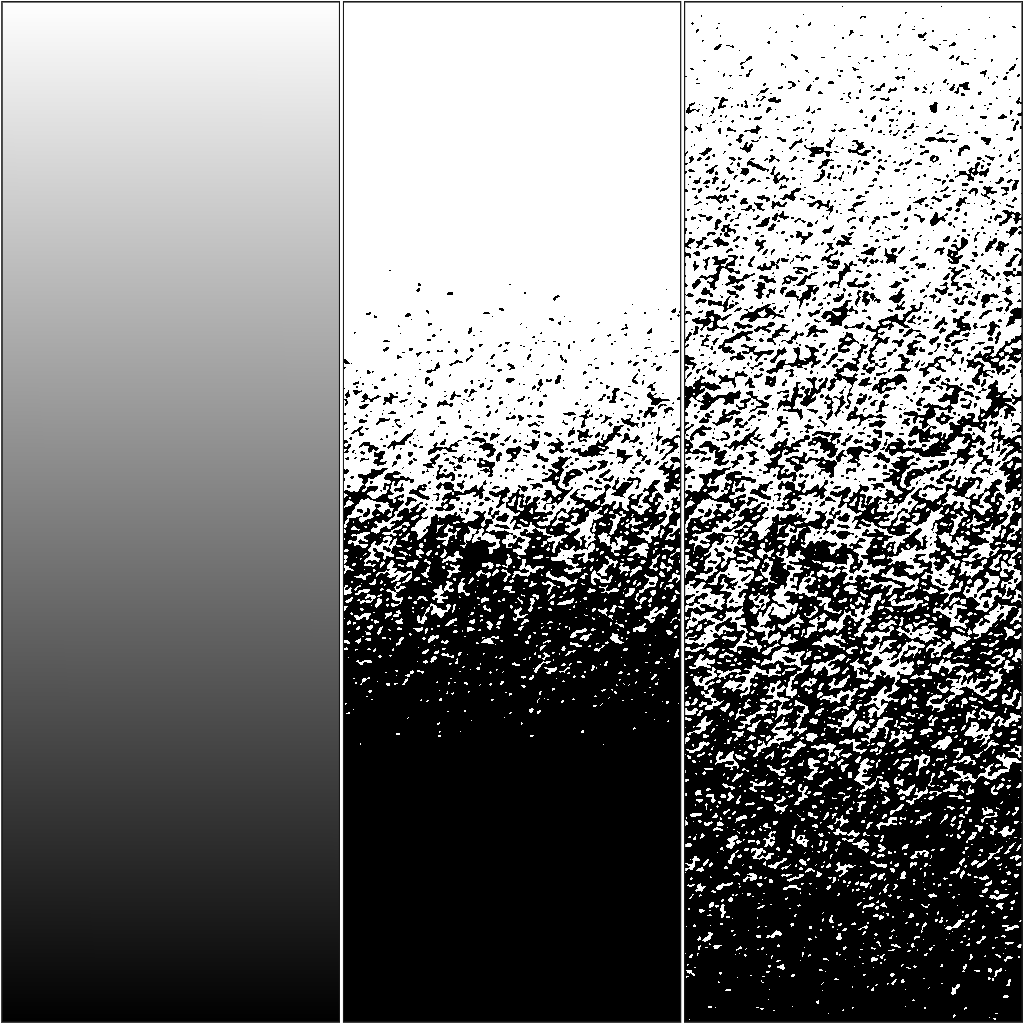
\includegraphics[width=0.5\textwidth]{fig/Mix-Max/Priority W1.png}
    \\
    \begin{tabular}{
        >{\centering\arraybackslash}m{0.13\textwidth}
        >{\centering\arraybackslash}m{0.13\textwidth}
        >{\centering\arraybackslash}m{0.13\textwidth}
        }

        \footnotesize $v_1$               &
        \footnotesize $w_1$ \cite{mixmax} &
        \footnotesize $w_1$ équilibré
    \end{tabular}

    \caption{
        Comparaison de l'équilibrage de la méthode Mix-Max entre deux textures procédurales similaires (Local Random Phase Noise \cite{LRPN}) à histogramme gaussien. La première colonne montre le poids original. La seconde colonne montre l'opacité générée par le Mix-Max \cite{mixmax} vu à l'équation \ref{Bases Mix Max}. La dernière colonne montre l'opacité généré par le Mix-Max équilibré utilisant le décallage vu à l'équation \ref{Formule Delta Mix Max Equilibré} ainsi qu'un applatissement d'histogramme des priorités. L'équilibre du mélange final est bien visible dans la répartition de l'opacité qui suit correctement le poids initial.
    }
    \label{Résultats Priorités}
\end{figure}

\subsection{Priorité de bruits procéduraux}

L'applatissement de priorité matricielle n'est qu'une étape de pré-traitement
simple à effectuer. Cependant, l'utilisation d'un bruit procédural en texture
de priorité nécéssite un applatissement en temps réel de ce dernier.

Une telle opération est réalisable à l'aide de la fonction de répartition
$F_{\mathcal{B}}$ du bruit $\mathcal{B}$. Une version uniformément distribué de
ce bruit $\mathcal{U}$ est alors obtenable à l'aide de la formule :
\begin{equation}\centering\label{Unfirmisation procédurale}
    \mathcal{U}(\mathbf{u}) = F_{\mathcal{B}}(\mathcal{B}(\mathbf{u}))
\end{equation}
La fonction de répartition de n'importe quelle texture peut être obtenue en intégran son histogramme. Dans mon implémentation, une discrétisation de cette fonction sur 16 à 32 points, obtenus en sommant les valeurs de l'histogramme, est suffisante pour obtenir de bons réusltats. Cette formule convient à n'importe quel bruit procédural stationnaire. La figure \ref{Résultats Priorités} montre les résultats obtenus avec cette méthode.

\subsection{Micro-priorité et filtrage pour un mélange équilibré}

Afin d'utiliser l'opérateur Mix-Max pour créer des textures affichés à l'écran,
il est nécéssaire d'avoir une méthode de filtrage analytique. Pour cela, le
papier original \cite{mixmax} a introduit une équation permettant de calculer
l'empreinte de l'opacité d'une texture sur une zone $\mathbb{P}$ :
\begin{equation}\centering\label{FS24_micro-priorite}
    w_1(\mathbb{P}) = 1 - \Phi \left(
    \frac{
            \mathcal{S}_2(\mathbb{P}) + v_2(\mathbb{P}) - \mathcal{S}_2(\mathbb{P}) + v_2(\mathbb{P})
        }{
            \sqrt{\sigma_1^2 + \sigma_2^2 + \lambda_1^2 + \lambda_2^2}
        }
    \right)
\end{equation}
Où $\Phi$ est la fonction de répartition de la loi normale standard, $\sigma_i^2$ la variance de la texture $\mathcal{S}_i$ sur la zone $\mathbb{P}$ et $\lambda_1$ la micro-priorité (ou variance de base) de la texutre, utilisée pour représenter les micro-détails de la texture en lissant le mélange.

Cependant, lorsque l'on applique l'applatissement de l'histogramme de la
priorité et le décallage $\Delta_i$ vu à l'équation \ref{Formule Delta Mix Max
    Equilibré}, le résultat n'est pas équilibré.

\begin{figure}
    \centering

    \begin{tabular}{c | c}
        \begin{tikzpicture}
            \begin{axis}[
                    title = \footnotesize Méthode (\ref{FS24_micro-priorite}) sans uniformisation,
                    view={-45}{45},
                    xlabel = $\sqrt{\lambda_1^2 + \lambda_2^2}$,
                    ylabel = $v_1$,
                    zlabel = $w_1(\mathbb{P})$,
                    xlabel style={sloped like x axis},
                    ylabel style={sloped}
                ]
                \addplot3[
                    surf,
                    colormap/greenyellow
                ]
                % (Longueur, profondeur, hauteur)
                % (Lambda, Alpha, Présence)
                coordinates { (0,0,0) (0,0.125,0.023) (0, 0.25, 0.07) (0, 0.375, 0.23) (0, 0.5,
                        0.5) (0, 0.625, 0.77) (0, 0.75, 0.91) (0, 1, 1)

                        (0.5,0,0) (0.5,0.125,0.07) (0.5, 0.25, 0.15) (0.5, 0.375, 0.3) (0.5, 0.5, 0.5) (0.5, 0.625, 0.70) (0.5, 0.75, 0.84) (0.5, 1, 1)

                        (1,0,0) (1,0.125,0.165) (1, 0.25, 0.25) (1, 0.375, 0.36) (1, 0.5, 0.5) (1, 0.625, 0.63) (1, 0.75, 0.74) (1, 1, 1)
                    };
            \end{axis}
        \end{tikzpicture}
         &
        \begin{tikzpicture}
            \begin{axis}[
                    title = \footnotesize Méthode (\ref{FS24_micro-priorite}) avec uniformisation (\ref{20}),
                    view={-45}{45},
                    xlabel = $\sqrt{\lambda_1^2 + \lambda_2^2}$,
                    ylabel = $v_1$,
                    zlabel = $w_1(\mathbb{P})$,
                    xlabel style={sloped like x axis},
                    ylabel style={sloped}
                ]
                \addplot3[
                    surf,
                    colormap/redyellow,
                ]
                % (Longueur, profondeur, hauteur)
                % (Lambda, Alpha, Présence)
                coordinates { (0,0,0) (0,0.125,0.1) (0, 0.25, 0.23) (0, 0.375, 0.37) (0, 0.5,
                        0.5) (0, 0.625, 0.63) (0, 0.75, 0.77) (0, 1, 1)

                        (0.5,0,0) (0.5,0.125,0.12) (0.5, 0.25, 0.24) (0.5, 0.375, 0.374) (0.5, 0.5, 0.5) (0.5, 0.625, 0.624) (0.5, 0.75, 0.77) (0.5, 1, 1)

                        (1,0,0) (1,0.125,0.14) (1, 0.25, 0.26) (1, 0.375, 0.38) (1, 0.5, 0.5) (1, 0.625, 0.615) (1, 0.75, 0.74) (1, 1, 1)
                    };
            \end{axis}
        \end{tikzpicture}

    \end{tabular}

    \caption{Caption}
    \label{fig:enter-label}
\end{figure}

\subsection{Méthode d'estimation de la variance de textures procédurales}

\section{Conclusion et apports}

\subsection{Pavage et mélange}

\subsection{Mix-Max}

\subsection{Perspectives et améliorations}

\clearpage

\printbibliography

\end{document}